\noautobookmark
\begin{frame}[t]{ASE reduces stored energy in laser gain media}
  \movie[
  width = 0.8\paperwidth,
  height = 0.7\textheight,
  %showcontrols = true,
  autostart = false,
  loop,
  play,
  pause,
  resume
  ]       
  {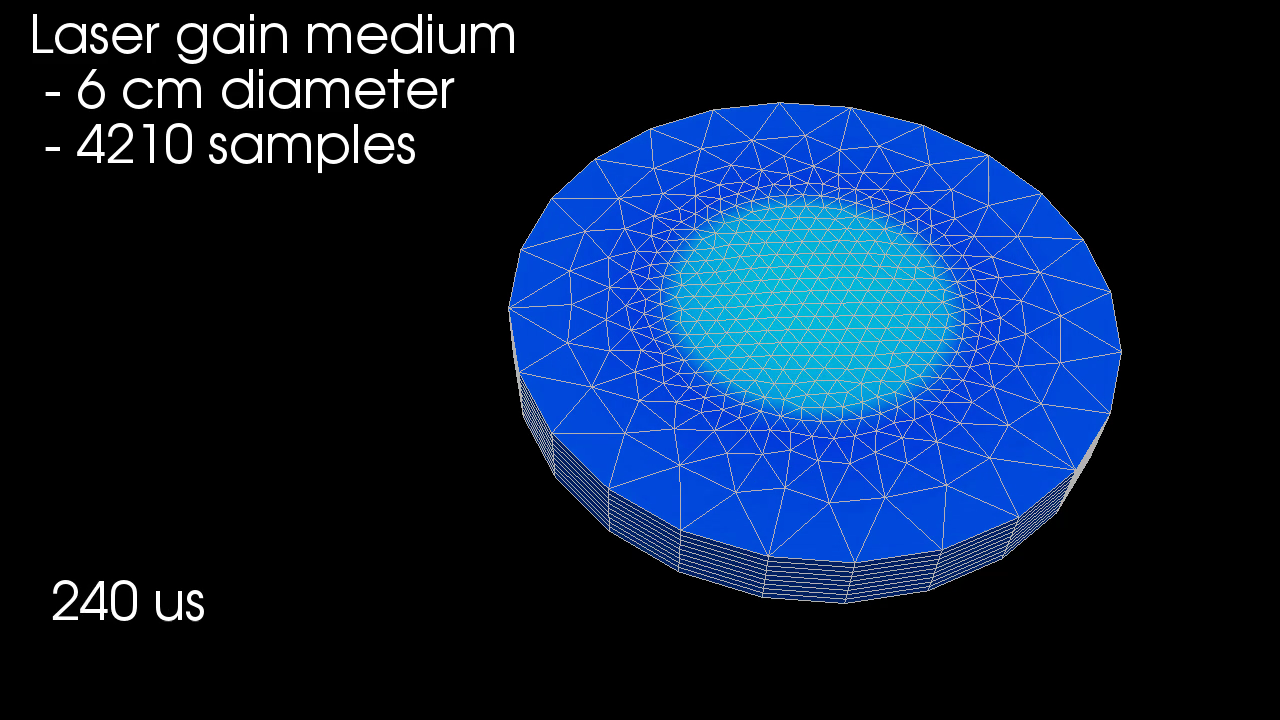
\includegraphics[width=.8\paperwidth, height=.7\textheight]{animation_talk_720c_new.png}}{animation_talk_720c_new.avi}

%
%  \begin{columns}[T]
%
%    \begin{column}{.5\textwidth}
%      \textbf{graphic: ASE crystal, with a photon travelling through it?}\\[2ex]
%      \textbf{alternative: laser setup, pumping a gain medium?}
%    \end{column}
%
%    \begin{column}{.5\textwidth}
%      \begin{itemize}
%      \myuncover{1}{3}{
%        \item In laser physics, gain media are pumped by lasers\\[1ex]
%      }
%      \myuncover{2}{3}{
%        \item Over time, electrons fall back into lower energy levels, causing
%          the spontaneous emission of a photon\\[1ex]
%      }
%      \myuncover{3}{3}{
%        \item Photon travels through the medium, where it is amplified by more
%          photons that are released
%      }
%  \end{itemize}
%    \end{column}
%
%  \end{columns}
\end{frame}
